\documentclass{standalone}
\usepackage{tikz}
\usetikzlibrary{patterns, positioning}


\begin{document}
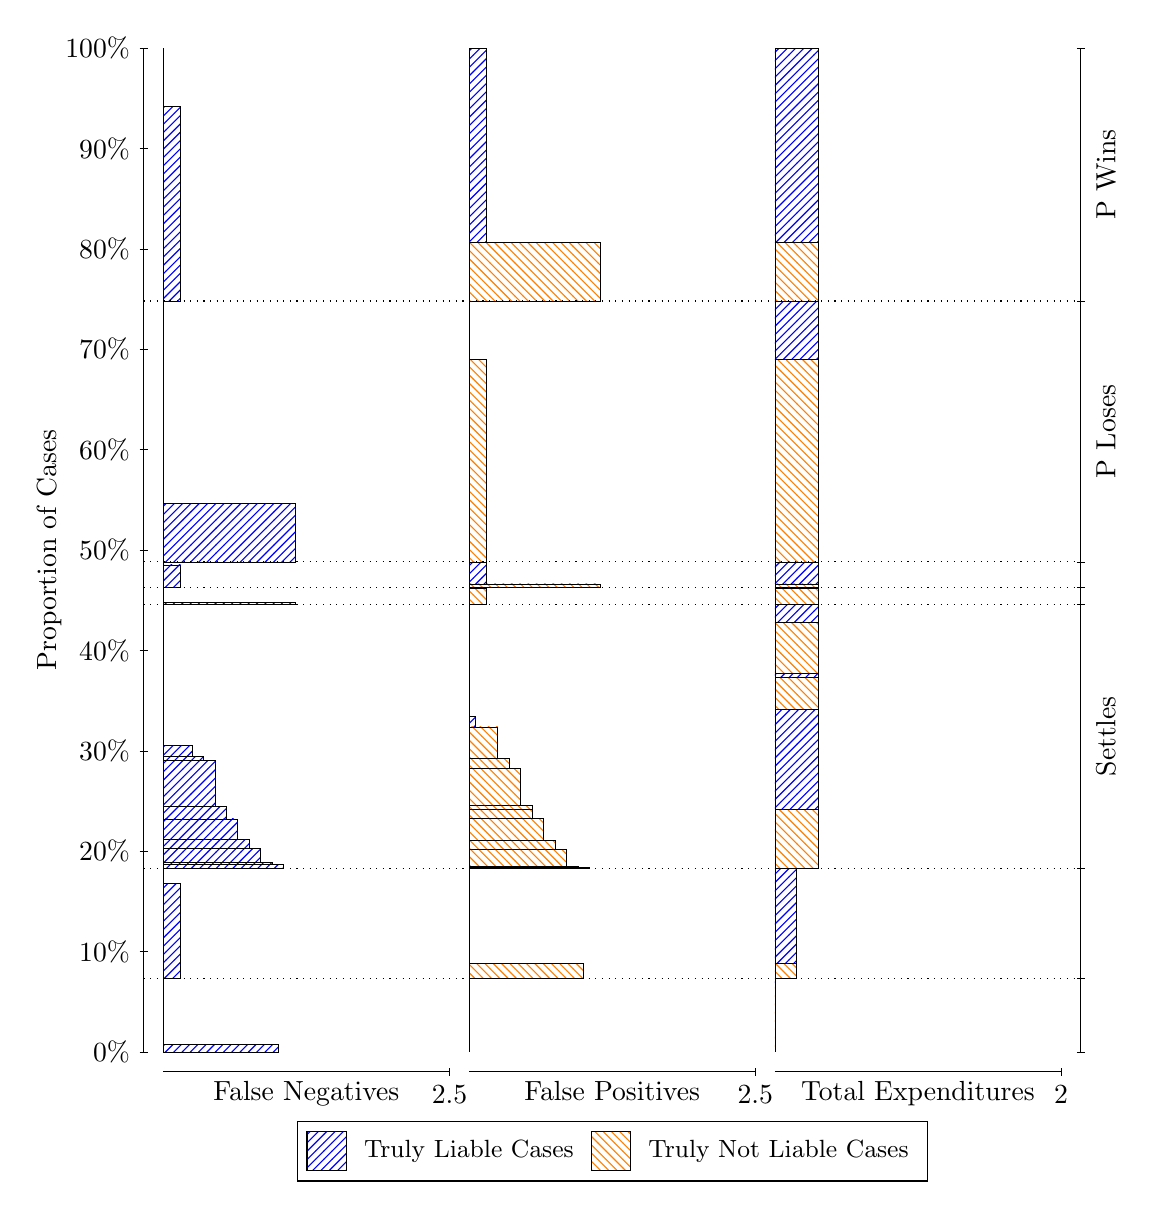
\begin{tikzpicture}
\draw[black, very thin] (1.5,1.75) -- (1.5,14.5);
\node[rotate=90, text=black, anchor=center] at (0.3, 8.125) {Proportion of Cases};
\draw[black, very thin] (1.45,1.75) -- (1.55,1.75);
\node[text=black, anchor=east] at (1.45, 1.75) {0\%};
\draw[black, very thin] (1.45,3.025) -- (1.55,3.025);
\node[text=black, anchor=east] at (1.45, 3.025) {10\%};
\draw[black, very thin] (1.45,4.3) -- (1.55,4.3);
\node[text=black, anchor=east] at (1.45, 4.3) {20\%};
\draw[black, very thin] (1.45,5.575) -- (1.55,5.575);
\node[text=black, anchor=east] at (1.45, 5.575) {30\%};
\draw[black, very thin] (1.45,6.85) -- (1.55,6.85);
\node[text=black, anchor=east] at (1.45, 6.85) {40\%};
\draw[black, very thin] (1.45,8.125) -- (1.55,8.125);
\node[text=black, anchor=east] at (1.45, 8.125) {50\%};
\draw[black, very thin] (1.45,9.4) -- (1.55,9.4);
\node[text=black, anchor=east] at (1.45, 9.4) {60\%};
\draw[black, very thin] (1.45,10.675) -- (1.55,10.675);
\node[text=black, anchor=east] at (1.45, 10.675) {70\%};
\draw[black, very thin] (1.45,11.95) -- (1.55,11.95);
\node[text=black, anchor=east] at (1.45, 11.95) {80\%};
\draw[black, very thin] (1.45,13.225) -- (1.55,13.225);
\node[text=black, anchor=east] at (1.45, 13.225) {90\%};
\draw[black, very thin] (1.45,14.5) -- (1.55,14.5);
\node[text=black, anchor=east] at (1.45, 14.5) {100\%};

\draw[black, very thin] (13.4,1.75) -- (13.4,14.5);
\draw[black, very thin] (13.35,1.75) -- (13.45,1.75);
\node[anchor=west] at (13.35, 1.75) {};
\draw[black, very thin] (13.35,2.687) -- (13.45,2.687);
\node[anchor=west] at (13.35, 2.687) {};
\draw[black, very thin] (13.35,4.0833) -- (13.45,4.0833);
\node[anchor=west] at (13.35, 4.0833) {};
\draw[black, very thin] (13.35,7.4361) -- (13.45,7.4361);
\node[anchor=west] at (13.35, 7.4361) {};
\draw[black, very thin] (13.35,7.6541) -- (13.45,7.6541);
\node[anchor=west] at (13.35, 7.6541) {};
\draw[black, very thin] (13.35,7.975) -- (13.45,7.975);
\node[anchor=west] at (13.35, 7.975) {};
\draw[black, very thin] (13.35,11.287) -- (13.45,11.287);
\node[anchor=west] at (13.35, 11.287) {};
\draw[black, very thin] (13.35,14.5) -- (13.45,14.5);
\node[anchor=west] at (13.35, 14.5) {};

\draw[black, very thin, pattern color=blue, pattern=north east lines] (1.75,1.75) rectangle (3.2033,1.8486);
\draw[black, very thin, pattern color=orange, pattern=north west lines] (1.75,1.8486) rectangle (1.75,2.687);
\draw[black, very thin, pattern color=blue, pattern=north east lines] (1.75,2.687) rectangle (1.968,3.892);
\draw[black, very thin, pattern color=orange, pattern=north west lines] (1.75,3.892) rectangle (1.75,4.0833);
\draw[black, very thin, pattern color=blue, pattern=north east lines] (1.75,4.0833) rectangle (3.276,4.1329);
\draw[black, very thin, pattern color=blue, pattern=north east lines] (1.75,4.1329) rectangle (3.1307,4.1625);
\draw[black, very thin, pattern color=blue, pattern=north east lines] (1.75,4.1625) rectangle (2.9853,4.3364);
\draw[black, very thin, pattern color=blue, pattern=north east lines] (1.75,4.3364) rectangle (2.84,4.4484);
\draw[black, very thin, pattern color=blue, pattern=north east lines] (1.75,4.4484) rectangle (2.6947,4.7103);
\draw[black, very thin, pattern color=blue, pattern=north east lines] (1.75,4.7103) rectangle (2.5493,4.8642);
\draw[black, very thin, pattern color=blue, pattern=north east lines] (1.75,4.8642) rectangle (2.404,5.4511);
\draw[black, very thin, pattern color=blue, pattern=north east lines] (1.75,5.4511) rectangle (2.2587,5.508);
\draw[black, very thin, pattern color=blue, pattern=north east lines] (1.75,5.508) rectangle (2.1133,5.64);
\draw[black, very thin, pattern color=orange, pattern=north west lines] (1.75,5.64) rectangle (1.75,7.4361);
\draw[black, very thin, pattern color=blue, pattern=north east lines] (1.75,7.4361) rectangle (3.4213,7.4559);
\draw[black, very thin, pattern color=orange, pattern=north west lines] (1.75,7.4559) rectangle (1.75,7.6541);
\draw[black, very thin, pattern color=blue, pattern=north east lines] (1.75,7.6541) rectangle (1.968,7.9358);
\draw[black, very thin, pattern color=orange, pattern=north west lines] (1.75,7.9358) rectangle (1.75,7.975);
\draw[black, very thin, pattern color=blue, pattern=north east lines] (1.75,7.975) rectangle (3.4213,8.7204);
\draw[black, very thin, pattern color=orange, pattern=north west lines] (1.75,8.7204) rectangle (1.75,11.287);
\draw[black, very thin, pattern color=blue, pattern=north east lines] (1.75,11.287) rectangle (1.968,13.755);
\draw[black, very thin, pattern color=orange, pattern=north west lines] (1.75,13.755) rectangle (1.75,14.5);
\draw[black, very thin, pattern color=orange, pattern=north west lines] (5.6333,1.75) rectangle (5.6333,2.5884);
\draw[black, very thin, pattern color=blue, pattern=north east lines] (5.6333,2.5884) rectangle (5.6333,2.687);
\draw[black, very thin, pattern color=orange, pattern=north west lines] (5.6333,2.687) rectangle (7.0867,2.8783);
\draw[black, very thin, pattern color=blue, pattern=north east lines] (5.6333,2.8783) rectangle (5.6333,4.0833);
\draw[black, very thin, pattern color=orange, pattern=north west lines] (5.6333,4.0833) rectangle (7.1593,4.0973);
\draw[black, very thin, pattern color=orange, pattern=north west lines] (5.6333,4.0973) rectangle (7.014,4.1083);
\draw[black, very thin, pattern color=orange, pattern=north west lines] (5.6333,4.1083) rectangle (6.8687,4.3256);
\draw[black, very thin, pattern color=orange, pattern=north west lines] (5.6333,4.3256) rectangle (6.7233,4.4408);
\draw[black, very thin, pattern color=orange, pattern=north west lines] (5.6333,4.4408) rectangle (6.578,4.7197);
\draw[black, very thin, pattern color=orange, pattern=north west lines] (5.6333,4.7197) rectangle (6.4327,4.8301);
\draw[black, very thin, pattern color=orange, pattern=north west lines] (5.6333,4.8301) rectangle (6.4327,4.8849);
\draw[black, very thin, pattern color=orange, pattern=north west lines] (5.6333,4.8849) rectangle (6.2873,5.3522);
\draw[black, very thin, pattern color=orange, pattern=north west lines] (5.6333,5.3522) rectangle (6.142,5.4798);
\draw[black, very thin, pattern color=orange, pattern=north west lines] (5.6333,5.4798) rectangle (5.9967,5.8793);
\draw[black, very thin, pattern color=blue, pattern=north east lines] (5.6333,5.8793) rectangle (5.706,6.0113);
\draw[black, very thin, pattern color=blue, pattern=north east lines] (5.6333,6.0113) rectangle (5.6333,7.4361);
\draw[black, very thin, pattern color=orange, pattern=north west lines] (5.6333,7.4361) rectangle (5.8513,7.6342);
\draw[black, very thin, pattern color=blue, pattern=north east lines] (5.6333,7.6342) rectangle (5.6333,7.6541);
\draw[black, very thin, pattern color=orange, pattern=north west lines] (5.6333,7.6541) rectangle (7.3047,7.6933);
\draw[black, very thin, pattern color=blue, pattern=north east lines] (5.6333,7.6933) rectangle (5.8513,7.975);
\draw[black, very thin, pattern color=orange, pattern=north west lines] (5.6333,7.975) rectangle (5.8513,10.542);
\draw[black, very thin, pattern color=blue, pattern=north east lines] (5.6333,10.542) rectangle (5.6333,11.287);
\draw[black, very thin, pattern color=orange, pattern=north west lines] (5.6333,11.287) rectangle (7.3047,12.032);
\draw[black, very thin, pattern color=blue, pattern=north east lines] (5.6333,12.032) rectangle (5.8513,14.5);
\draw[black, very thin, pattern color=orange, pattern=north west lines] (9.5167,1.75) rectangle (9.5167,2.5884);
\draw[black, very thin, pattern color=blue, pattern=north east lines] (9.5167,2.5884) rectangle (9.5167,2.687);
\draw[black, very thin, pattern color=orange, pattern=north west lines] (9.5167,2.687) rectangle (9.7892,2.8783);
\draw[black, very thin, pattern color=blue, pattern=north east lines] (9.5167,2.8783) rectangle (9.7892,4.0833);
\draw[black, very thin, pattern color=orange, pattern=north west lines] (9.5167,4.0833) rectangle (10.062,4.8301);
\draw[black, very thin, pattern color=blue, pattern=north east lines] (9.5167,4.8301) rectangle (10.062,6.1046);
\draw[black, very thin, pattern color=orange, pattern=north west lines] (9.5167,6.1046) rectangle (10.062,6.5041);
\draw[black, very thin, pattern color=blue, pattern=north east lines] (9.5167,6.5041) rectangle (10.062,6.5537);
\draw[black, very thin, pattern color=orange, pattern=north west lines] (9.5167,6.5537) rectangle (10.062,7.2035);
\draw[black, very thin, pattern color=blue, pattern=north east lines] (9.5167,7.2035) rectangle (10.062,7.4361);
\draw[black, very thin, pattern color=orange, pattern=north west lines] (9.5167,7.4361) rectangle (10.062,7.6342);
\draw[black, very thin, pattern color=blue, pattern=north east lines] (9.5167,7.6342) rectangle (10.062,7.6541);
\draw[black, very thin, pattern color=orange, pattern=north west lines] (9.5167,7.6541) rectangle (10.062,7.6933);
\draw[black, very thin, pattern color=blue, pattern=north east lines] (9.5167,7.6933) rectangle (10.062,7.975);
\draw[black, very thin, pattern color=orange, pattern=north west lines] (9.5167,7.975) rectangle (10.062,10.542);
\draw[black, very thin, pattern color=blue, pattern=north east lines] (9.5167,10.542) rectangle (10.062,11.287);
\draw[black, very thin, pattern color=orange, pattern=north west lines] (9.5167,11.287) rectangle (10.062,12.032);
\draw[black, very thin, pattern color=blue, pattern=north east lines] (9.5167,12.032) rectangle (10.062,14.5);
\draw[black, dotted] (1.5,2.687) -- (13.4,2.687);
\draw[black, dotted] (1.5,4.0833) -- (13.4,4.0833);
\draw[black, dotted] (1.5,7.4361) -- (13.4,7.4361);
\draw[black, dotted] (1.5,7.6541) -- (13.4,7.6541);
\draw[black, dotted] (1.5,7.975) -- (13.4,7.975);
\draw[black, dotted] (1.5,11.287) -- (13.4,11.287);
\draw[black, very thin] (1.75,1.5) -- (5.3833,1.5);
\node[text=black, anchor=north] at (3.5667, 1.5) {False Negatives};
\draw[black, very thin] (5.3833,1.45) -- (5.3833,1.55);
\node[text=black, anchor=north] at (5.3833, 1.45) {2.5};

\draw[black, very thin] (5.6333,1.5) -- (9.2667,1.5);
\node[text=black, anchor=north] at (7.45, 1.5) {False Positives};
\draw[black, very thin] (9.2667,1.45) -- (9.2667,1.55);
\node[text=black, anchor=north] at (9.2667, 1.45) {2.5};

\draw[black, very thin] (9.5167,1.5) -- (13.15,1.5);
\node[text=black, anchor=north] at (11.333, 1.5) {Total Expenditures};
\draw[black, very thin] (13.15,1.45) -- (13.15,1.55);
\node[text=black, anchor=north] at (13.15, 1.45) {2};



\node[text=black, centered, rotate=90] at (13.72, 5.7597) {Settles};


\node[text=black, centered, rotate=90] at (13.72, 9.6312) {P Loses};
\node[text=black, centered, rotate=90] at (13.72, 12.894) {P Wins};

\draw (7.449999999999999,1.5) node[draw=none] (baseCoordinate) {};
\begin{scope}[align=center]
        \matrix[scale=0.5, draw=black, below=0.5cm of baseCoordinate, nodes={draw}, column sep=0.1cm]{
            \node[rectangle, draw, minimum width=0.5cm, minimum height=0.5cm, pattern color=blue, pattern=north east lines] {}; &
            \node[draw=none, font=\small, text=black] (B) {Truly Liable Cases}; &
            \node[rectangle, draw, minimum width=0.5cm, minimum height=0.5cm, pattern color=orange, pattern=north west lines] {}; &
            \node[draw=none, font=\small, text=black] (B) {Truly Not Liable Cases}; \\
            };
\end{scope}

\end{tikzpicture}
\end{document}